\subsection{Observations and Motivation} % just find the problem and benefit
\label{sec:observationandmotivation}

%\subsection{Need for Deduplication}

%The proliferation of Containers and Container platforms has resulted in an explosion of the number of Docker images.
%In order to understand the extent of storage requirements and performance demands from a Docker registry, 
%we observe the amount of public repositories hosted by Docker Hub registry. 
%We chose the Docker Hub registry~\cite{docker-hub} as our source of images due to its popularity 
%and its significant number of public repositories. 
%%
%Docker Hub does not provide an API to retrieve all repository names.
%Hence, we crawled the registry's website to obtain a list of all available
%repositories, and then downloaded the \emph{latest} version of an image and its
%corresponding layers for each repository.
% over a period of 30 days.
%
%We plan to extend our analysis to other image tags in the future.
%
%We downloaded 355,319 images, resulting in 1,792,609 compressed layers
%and 5,278,465,130 files, with a total compressed dataset size of 47\,TB.
%
%
%To store and analyze the data, we deployed an 8-node Spark~\cite{spark}
%cluster with HDFS~\cite{hdfs} as the backend storage.
%%

\paragraph{Deduplication for Docker registries?}

%\subsection{Deduplication on cloud storage systems}

%Modern Docker registry identifies and addresses a layer with a digest that is computed based on the uncompressed layer's content (e.g., SHA-256).
%Identifying layers by their content allows the registry to store only one instance of a layer even if it is referenced by multiple images. 
%However, if at least one file differs in two otherwise identical layers, the two layers are treated as different and stored separately.
%\paragraph{Images and layers}

We observe that the number of public repositories in Docker Hub is constantly increasing with a growth that amounts 
to around 1 million repositories annually. Based on our estimation, this will cause at least~130\,TB of annual growth in storage needs.

On-cloud global deduplication software is widely adopted by cloud enterprises for reducing cloud storage consumption and overall storage cost. 
For example, StorReduce~\cite{storReduce}, the deduplication software choice of Google cloud and AWS, 
performs in-line data deduplication transparently and resides between the client's application and the hosting cloud storage.
%A number of deduplication methods focus on client-side data deduplication to ensure that only unique files are uploaded, 
%to save network bandwidth, by having the client send a duplicate check request~\cite{xxx}~\cite{xxx}. 
%For example, xxxx\NZ{Hadeel, can you add one example and few relatedwork citation?}. 
Intuitively, such deduplication technique can be leveraged to eliminate redundant data from the Docker image storage system.  
Except, the Docker image dataset is different from the common data stream. 
Docker images are \emph{compressed archival files}.
%Intuitively, registries can be deployed as a proxy cache to host frequently requested layers to speedup image pulls and improve performance 
%while the backend cloud storage can leverage deduplication to save storage space.
%However, there are several unique problems concerning the integration of caching and deduplication to the unique Docker registries workload: \textbf{compressed layers}. 
%We investigate the potential for data reduction in the Docker registry by estimating the efficacy of layer sharing and file-level deduplication.
%We noticed that the number of public repositories is constantly increasing with a growth that amounts 
%to around 1 million repositories annually. 
%This corresponds to~130\,TB of annual growth in storage needs 
%\HA{but it is actually less because of shared layers, right?}, 
%costing around~\$15,000 a month if Google Cloud Storage is used~\cite{GoogleCloudStoragePricing}.
%This growth implies significant benefits to data deduplication. 

We performed an in-depth and empirical analysis of file-level deduplication on container images. 
We analyzed around 47\,TB of compressed Docker images (167\,TB after decompression) collected from Docker Hub. 
%In order to provide insights in terms of the redundancy measure in the image dataset and the benefits of deduplication,
%we have to first decompress the layers included in the images. 
%The decompressed layer comprises a set of files. 
%The total number of files we observed amount to over 5 billion files.
Surprisingly, only around 3\% of the those files are unique while the rest are redundant copies. 
We can save around half of the storage space after removing the duplicate files.

To eliminate these redundant files from the compressed layer files, changes must be made to the deduplication method. 
Such changes should recognize the compression formats, perform decompression before feeding the data to a block-level or file-level deduplication process. 
Otherwise, the deduplication ratio would be very low since compressed files have a very low deduplication ratio~\cite{meister2012study}. %"GZip-compressed files deduplication ratio is only 5.7%"
Moreover for restoring a layer, the layer's
containing files should all be fetched from wherever they reside, as they are likely to be scattered across multiple servers, 
and then compressed together, which causes a considerable overhead on pull layer requests performance.

\HA{running five registries, replaying dal trace using trace replayer-cite, and since the replayer doesn't use real layers we randomly match the request to our dataset downloaded from docker hub. describe how we got these numbers. for dedup, we simply implemented a decompress/compress + file-level deduplication on backend storage systems, we use a CHT based distributed storage system. Figure~\ref{fig:avg_latency_dedup_nodedup}}
\begin{figure}[t]
	\centering
	%\scriptsize
	\begin{minipage}{0.225\textwidth}
		\centering
		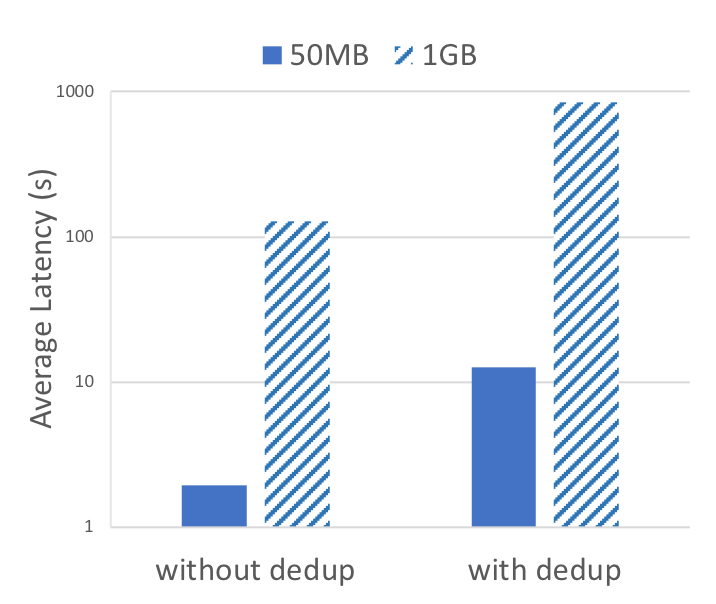
\includegraphics[width=1\textwidth]{graphs/avglatency_dedup_nodedup.png}
		\caption{Average latency.}
		\label{fig:avg_latency_dedup_nodedup}
	\end{minipage}
	\begin{minipage}{0.225\textwidth}
		\centering
		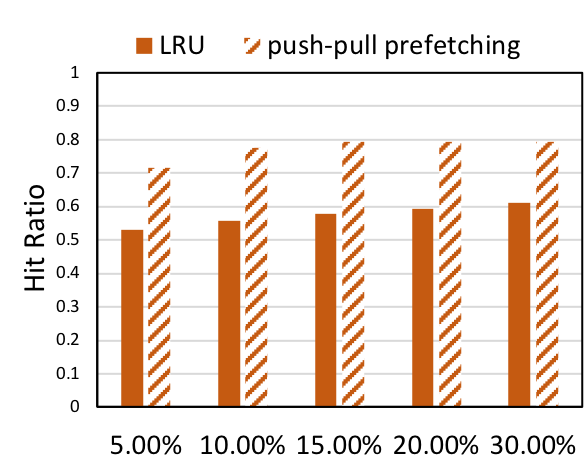
\includegraphics[width=1\textwidth]{graphs/lru_prefetch_hits.png}
		\caption{Hit ratio.}
		\vspace{-3pt}
		\label{fig:lru_prefetching_hits}
	\end{minipage}
\end{figure}
% for LRU and push-pull prefetching under different cache sizes (\% of total accessed layers).

\paragraph{Use registry as a web/proxy cache?}
Traditionally, caches are placed as close to the requesting client as possible, 
such caches are known as proxy caches, or web/HTTP caches for the temporary storage of 
frequently requested data to reduce the load on backend resources. 
For example, Varnish~\cite{varnish} and Squid~\cite{squid} are open-source high-performaning web/HTTP caches that accelerate web applications and improve response times by caching frequently requested web content.
%Examples of open-source web (HTTP) proxy caches include Nginx~\cite{?}, Squid~\cite{?}, and Varnish~\cite{?}. 
%They are typically implemented in an regional ISP or within a corporate network.
%Deduplication methods are implemented on remote backend storage servers, and
%transparently remove duplicates from the incoming data stream and restore the data for read requests. 
Docker registry is a web server that serves docker pull and docker push requests.
Intuitively, registries can be deployed as a proxy caches, \ie a pull-through cache~\cite{registryascache}, to host frequently requested layers to speedup image pulls and improve performance. 


%Caching is a technique widely leveraged to reduce bandwidth and load off of highly loaded bottleneck backends by temporarily storing frequently requested data~\cite{xxx}. 
%Caching can be introduced at the client, in between clients and servers as a proxy, or at the server side. 
%Proxy caches are efficient in reducing traffic from bottleneck backends by cooperatively serving previously requested and saved data without it going all they way to the backend~\cite{xxxx}. 
%Usually, caches are placed as close to the requesting client as possible, 
%such caches are known as proxy caches, or web/HTTP caches for the short-lived storage of 
%frequently requested/accessed data to reduce the server's lag. 

%The client therefore, experiences improved response times.
%The Docker client inherently caches layers at the client. This way, the Docker daemon only pulls layers that are not available on the host machine. 

%Other software used for caching include Memcached~\cite{?}, an open-source distributed in-memory key-value store that works as a caching system and Redis~\cite{?} which is an open-source key-value store that works as an in-memory store and as a cache
%\subsection{Apply traditional deduplication approaches to registries?}
%\subsection{Use-cases of \sysname}
%This suggests that the current layer sharing strategy that Docker already employs is not efficient in eliminating duplicate data. 
%Further investigations on the causes for the high number of redundant files exposed a few findings. 
%For example, different Docker images often contain the same 
%source code from external public repositories like GitHub~\cite{github}.
%This is because no official images contain this source code, 
%so users manually add it to their images, 
%resulting in different layers which cannot be reused.
%\paragraph{Deduplication statistics} % the potential of deduplication 

%%%%layer ref count 
%
%A remarkable observation that emerges from the data analysis is that only around 3\%\HA{3\% or 7\% ?} of the layers' constituent files are unique while the rest are redundant copies. 
%This suggests that the current layer sharing strategy that Docker already employs is not efficient in eliminating duplicate data. 
%We further analyzed the repeat count for every file and plotted the distributions as shown in Figure~\ref{fig:file-repeat-cnt}.
%We found that over 99.4\% of files have more than one copy.
%Around 50\% of files have exactly 4 copies and 90\% of files have 10 or less copies. 
%This indicates the high potential for file-level deduplication in the Docker registry.
%
%%\begin{figure} \centering
%	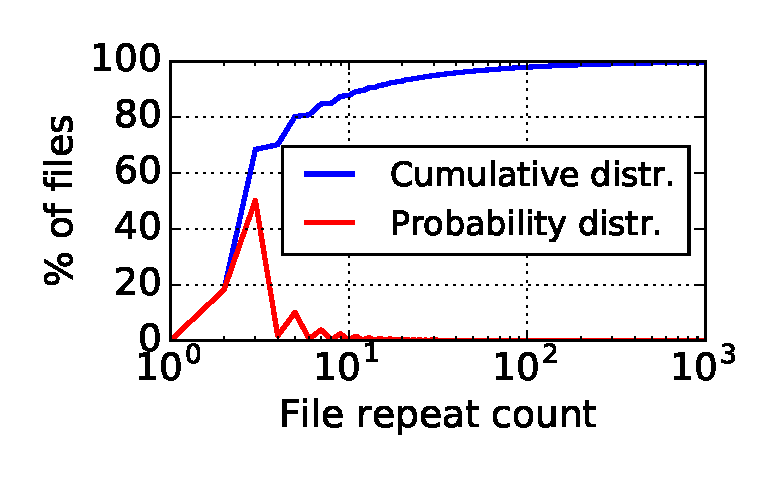
\includegraphics[width=0.45\textwidth]{graphs/File_repeat_count.eps}
%	\caption{File repeat count distribution.
%	%
%	\VT{No need for Y2}
%	%
%	\VT{Still need to use \% on the axis}\NZ{addressed both}
%	%
%	} \label{fig:file-repeat-cnt}
%\end{figure}

\begin{figure}[t]
	\centering
	\begin{minipage}{0.35\textwidth}
		\centering
		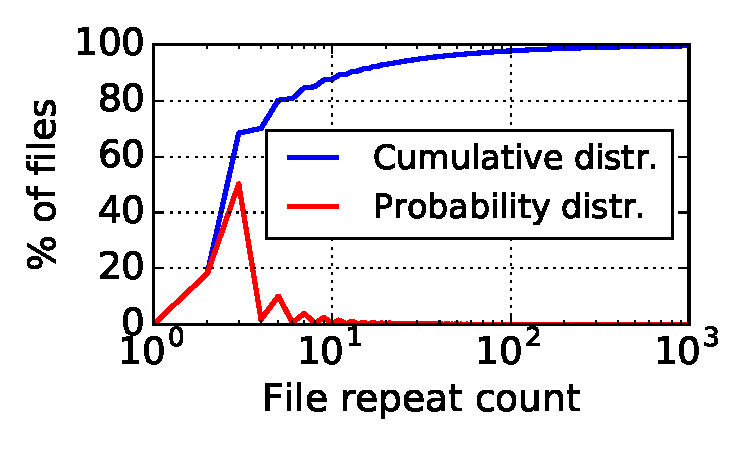
\includegraphics[width=1\textwidth]{graphs/File_repeat_count-eps.pdf}
		\caption{File repeat count distribution.
		}
		%\vspace{15pt}
		\label{fig:file-repeat-cnt}
	\end{minipage}
	\begin{minipage}{0.35\textwidth}
		\centering
		%\vspace{-10pt}
		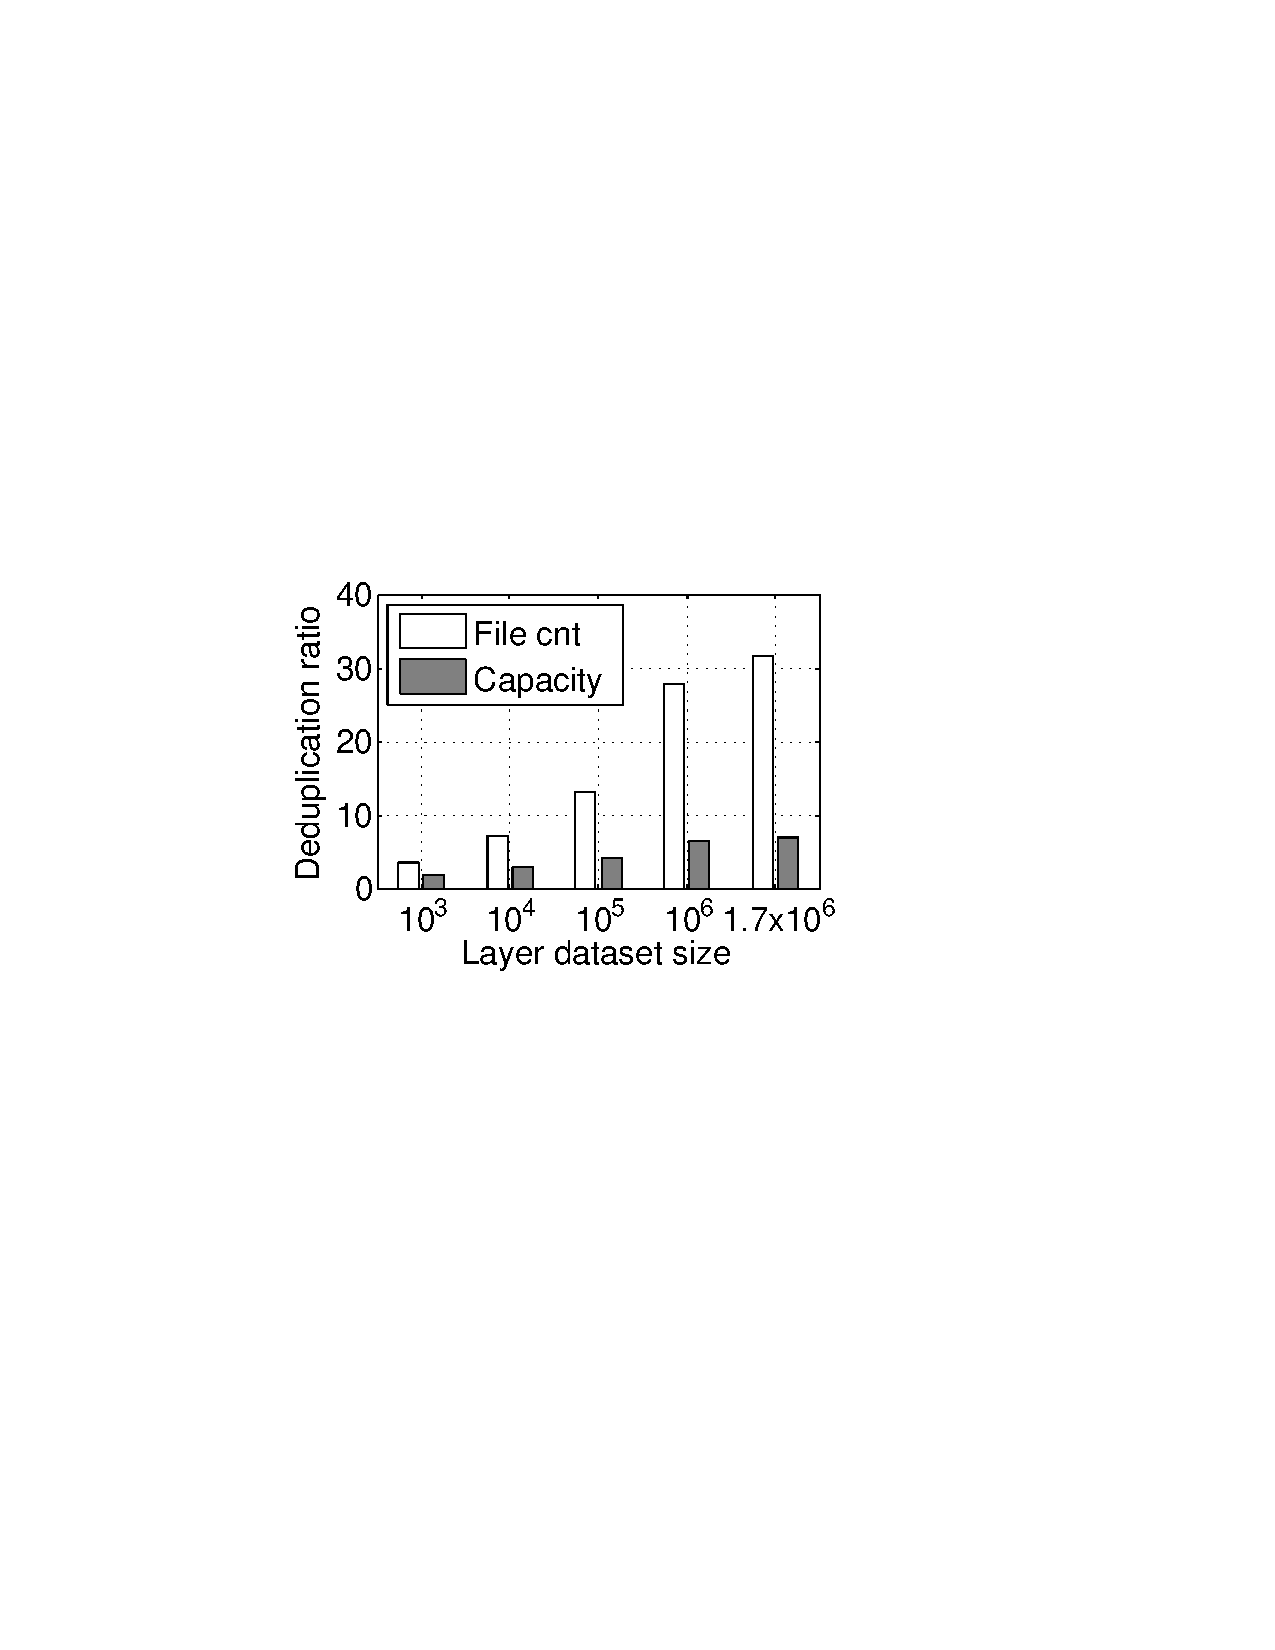
\includegraphics[width=1\textwidth]{graphs/dedup-ratio-grow} 
		\caption{Deduplication ratio growth.
		} 
		\vspace{-2pt}
		\label{fig:dedup-ratio-growth}
	\end{minipage}
\end{figure}

%\begin{figure} 
%	\centering
%	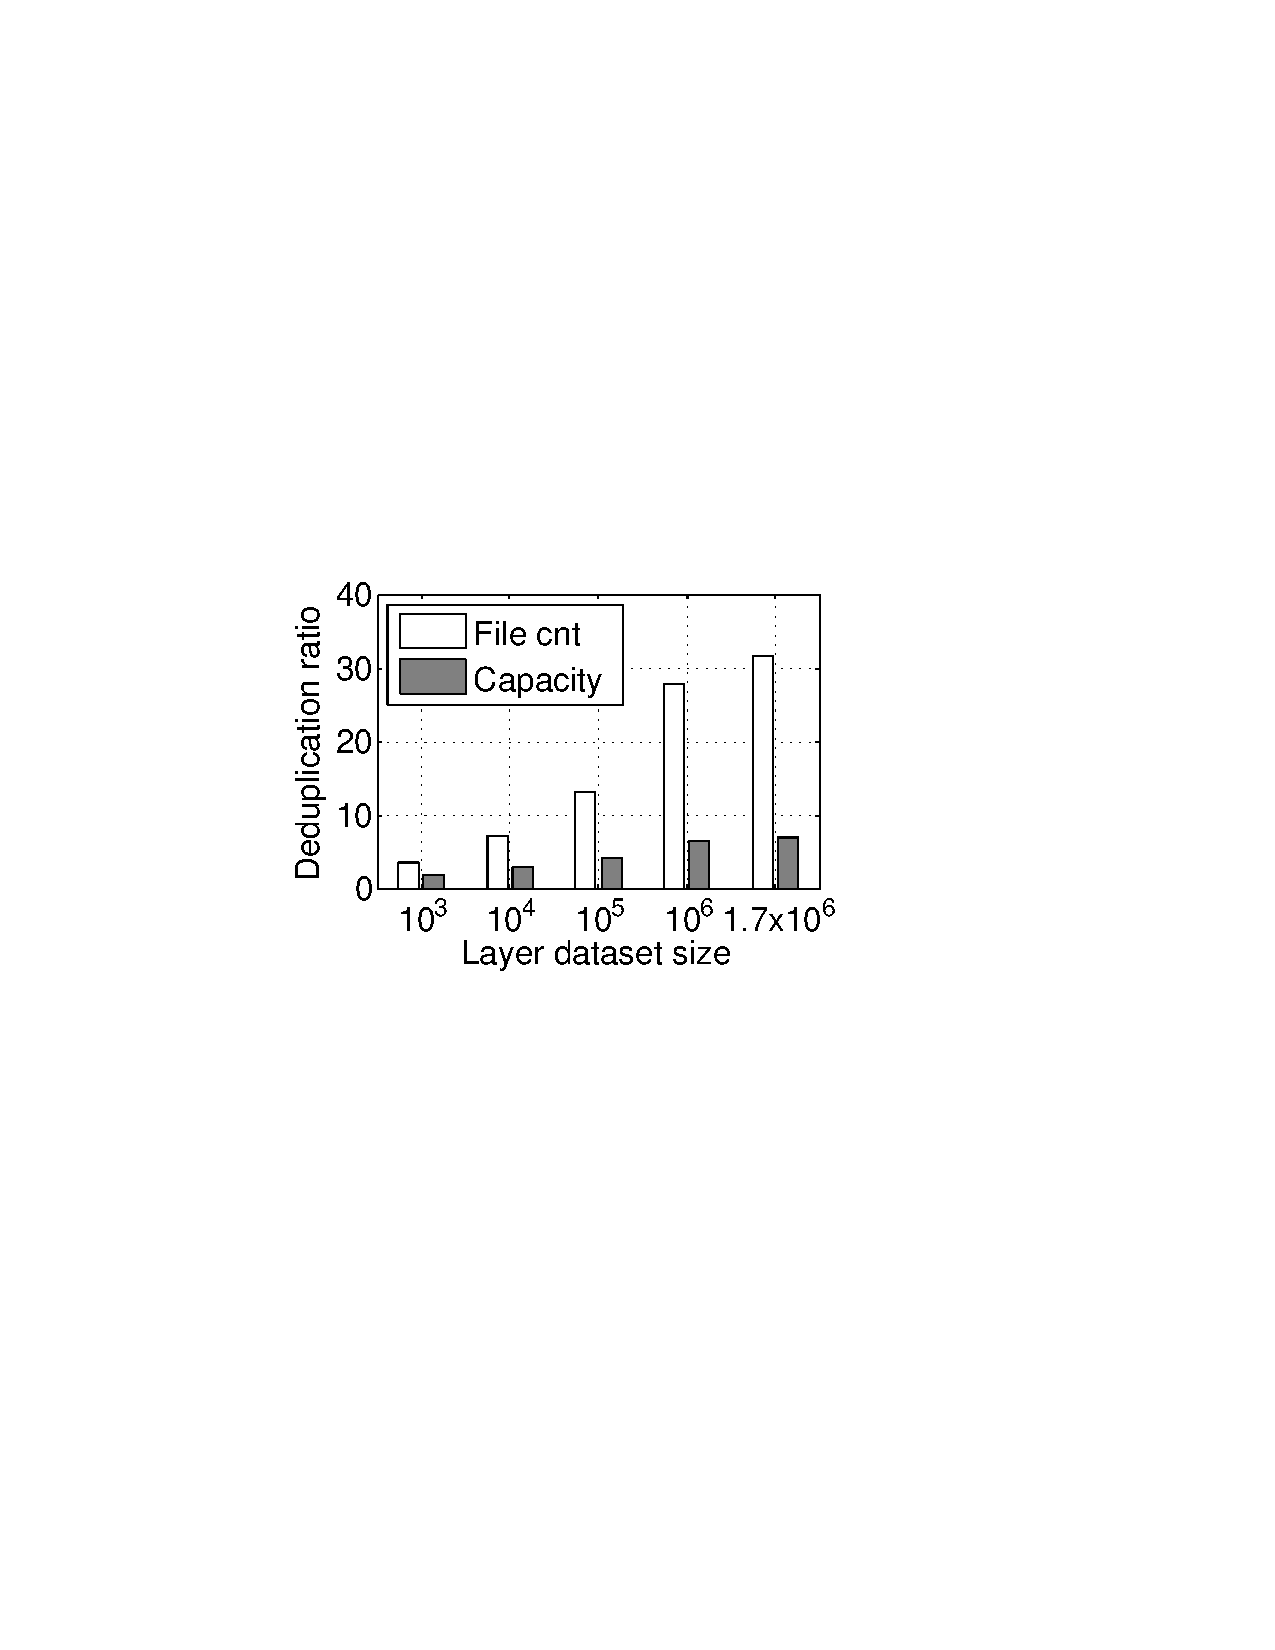
\includegraphics[width=0.25\textwidth]{graphs/dedup-ratio-grow} 
%	\caption{The growth of deduplication ratio.
%	} 
%	\label{fig:dedup-ratio-growth} 
%\end{figure}

%
%
%\paragraph{Deduplication ratio growth} % benefit
%%
%Further investigations on the potential of file-level deduplication involved analyzing the deduplication ratio. 
%As shown in Figure~\ref{fig:dedup-ratio-growth}, we analyzed the deduplication 
%ratio and its growth for an increasing number of files stored in the registry.   
%%(see Figure~\ref{fig:dedup-ratio-growth}).
%%
%%Figure~\ref{fig:dedup-ratio-growth} shows the deduplication ratio growth over the layer dataset size. 
%%
%The x-axis values correspond to the sizes of 4 random samples drawn from the whole dataset and the size of the
%whole dataset.
%
%We see that the deduplication ratio increases almost linearly with the layer dataset size.
%This implies that the benefits of file-level deduplication strengthens as the number of public repositories and images grow.
%
%As the number of images stored in the Docker registry increases dramatically,
%file-level deduplication can provide significant storage space savings.

%Intuitively, registries can be deployed as a proxy cache to host frequently requested layers to speedup image pulls and improve performance 
%while the backend cloud storage can leverage deduplication to save storage space.
%However, there are several unique problems concerning the integration of caching and deduplication to the unique Docker registries workload: \textbf{compressed layers}. 

%\subsection{Need for Usr-oriented cache management}
%
%\paragraph{Access skewness}
%
%\paragraph{Reuse time distribution}
%
%\paragraph{Hit ratios}
%
%\paragraph{Hit ratios with prefetching}
%
%%\subsection{} % what are the cost for a naive file-level deduplication
%
%\paragraph{Restoring performance breakdown}